% Options for packages loaded elsewhere
% Options for packages loaded elsewhere
\PassOptionsToPackage{unicode}{hyperref}
\PassOptionsToPackage{hyphens}{url}
\PassOptionsToPackage{dvipsnames,svgnames,x11names}{xcolor}
%
\documentclass[
  authoryear,
  preprint,
  3p,
  twocolumn]{elsarticle}
\usepackage{xcolor}
\usepackage{amsmath,amssymb}
\setcounter{secnumdepth}{5}
\usepackage{iftex}
\ifPDFTeX
  \usepackage[T1]{fontenc}
  \usepackage[utf8]{inputenc}
  \usepackage{textcomp} % provide euro and other symbols
\else % if luatex or xetex
  \usepackage{unicode-math} % this also loads fontspec
  \defaultfontfeatures{Scale=MatchLowercase}
  \defaultfontfeatures[\rmfamily]{Ligatures=TeX,Scale=1}
\fi
\usepackage{lmodern}
\ifPDFTeX\else
  % xetex/luatex font selection
\fi
% Use upquote if available, for straight quotes in verbatim environments
\IfFileExists{upquote.sty}{\usepackage{upquote}}{}
\IfFileExists{microtype.sty}{% use microtype if available
  \usepackage[]{microtype}
  \UseMicrotypeSet[protrusion]{basicmath} % disable protrusion for tt fonts
}{}
\makeatletter
\@ifundefined{KOMAClassName}{% if non-KOMA class
  \IfFileExists{parskip.sty}{%
    \usepackage{parskip}
  }{% else
    \setlength{\parindent}{0pt}
    \setlength{\parskip}{6pt plus 2pt minus 1pt}}
}{% if KOMA class
  \KOMAoptions{parskip=half}}
\makeatother
% Make \paragraph and \subparagraph free-standing
\makeatletter
\ifx\paragraph\undefined\else
  \let\oldparagraph\paragraph
  \renewcommand{\paragraph}{
    \@ifstar
      \xxxParagraphStar
      \xxxParagraphNoStar
  }
  \newcommand{\xxxParagraphStar}[1]{\oldparagraph*{#1}\mbox{}}
  \newcommand{\xxxParagraphNoStar}[1]{\oldparagraph{#1}\mbox{}}
\fi
\ifx\subparagraph\undefined\else
  \let\oldsubparagraph\subparagraph
  \renewcommand{\subparagraph}{
    \@ifstar
      \xxxSubParagraphStar
      \xxxSubParagraphNoStar
  }
  \newcommand{\xxxSubParagraphStar}[1]{\oldsubparagraph*{#1}\mbox{}}
  \newcommand{\xxxSubParagraphNoStar}[1]{\oldsubparagraph{#1}\mbox{}}
\fi
\makeatother


\usepackage{longtable,booktabs,array}
\usepackage{calc} % for calculating minipage widths
% Correct order of tables after \paragraph or \subparagraph
\usepackage{etoolbox}
\makeatletter
\patchcmd\longtable{\par}{\if@noskipsec\mbox{}\fi\par}{}{}
\makeatother
% Allow footnotes in longtable head/foot
\IfFileExists{footnotehyper.sty}{\usepackage{footnotehyper}}{\usepackage{footnote}}
\makesavenoteenv{longtable}
\usepackage{graphicx}
\makeatletter
\newsavebox\pandoc@box
\newcommand*\pandocbounded[1]{% scales image to fit in text height/width
  \sbox\pandoc@box{#1}%
  \Gscale@div\@tempa{\textheight}{\dimexpr\ht\pandoc@box+\dp\pandoc@box\relax}%
  \Gscale@div\@tempb{\linewidth}{\wd\pandoc@box}%
  \ifdim\@tempb\p@<\@tempa\p@\let\@tempa\@tempb\fi% select the smaller of both
  \ifdim\@tempa\p@<\p@\scalebox{\@tempa}{\usebox\pandoc@box}%
  \else\usebox{\pandoc@box}%
  \fi%
}
% Set default figure placement to htbp
\def\fps@figure{htbp}
\makeatother





\setlength{\emergencystretch}{3em} % prevent overfull lines

\providecommand{\tightlist}{%
  \setlength{\itemsep}{0pt}\setlength{\parskip}{0pt}}



 
\usepackage[]{natbib}
\bibliographystyle{elsarticle-harv}


\usepackage{amsmath,amssymb}
\usepackage{hyperref}
\usepackage{witharrows}
%\usepackage{natbib}
\usepackage{graphicx}
\usepackage{booktabs}
\usepackage{subcaption}
\usepackage{float}
\usepackage{placeins}
%\usepackage[minnames=1,maxnames=2,maxbibnames = 2, style=authoryear, bibstyle = authoryear, backend=bibtex, giveninits=true, block = none, isbn = false, url = false, doi = false, eprint = false]{biblatex}
\makeatletter
\@ifpackageloaded{caption}{}{\usepackage{caption}}
\AtBeginDocument{%
\ifdefined\contentsname
  \renewcommand*\contentsname{Table of contents}
\else
  \newcommand\contentsname{Table of contents}
\fi
\ifdefined\listfigurename
  \renewcommand*\listfigurename{List of Figures}
\else
  \newcommand\listfigurename{List of Figures}
\fi
\ifdefined\listtablename
  \renewcommand*\listtablename{List of Tables}
\else
  \newcommand\listtablename{List of Tables}
\fi
\ifdefined\figurename
  \renewcommand*\figurename{Figure}
\else
  \newcommand\figurename{Figure}
\fi
\ifdefined\tablename
  \renewcommand*\tablename{Table}
\else
  \newcommand\tablename{Table}
\fi
}
\@ifpackageloaded{float}{}{\usepackage{float}}
\floatstyle{ruled}
\@ifundefined{c@chapter}{\newfloat{codelisting}{h}{lop}}{\newfloat{codelisting}{h}{lop}[chapter]}
\floatname{codelisting}{Listing}
\newcommand*\listoflistings{\listof{codelisting}{List of Listings}}
\makeatother
\makeatletter
\makeatother
\makeatletter
\@ifpackageloaded{caption}{}{\usepackage{caption}}
\@ifpackageloaded{subcaption}{}{\usepackage{subcaption}}
\makeatother
\usepackage{float}
\makeatletter
\let\oldlt\longtable
\let\endoldlt\endlongtable
\def\longtable{\@ifnextchar[\longtable@i \longtable@ii}
\def\longtable@i[#1]{\begin{figure}[H]
\onecolumn
\begin{minipage}{0.5\textwidth}
\oldlt[#1]
}
\def\longtable@ii{\begin{figure}[H]
\onecolumn
\begin{minipage}{0.5\textwidth}
\oldlt
}
\def\endlongtable{\endoldlt
\end{minipage}
\twocolumn
\end{figure}}
\makeatother
\journal{Study of the correlation function}
\usepackage{bookmark}
\IfFileExists{xurl.sty}{\usepackage{xurl}}{} % add URL line breaks if available
\urlstyle{same}
\hypersetup{
  pdftitle={Large-Angle Statistics of the CMB Angular Correlation Function: Testing \textbackslash LambdaCDM at Low Multipoles},
  pdfauthor={Álvaro Méndez Rodríguez de Tembleque; Yago Ascasibar Sequeiros},
  pdfkeywords={cosmic microwave background, angular correlation
function, large-angle anomalies, Planck, \(\Lambda\)CDM},
  colorlinks=true,
  linkcolor={blue},
  filecolor={Maroon},
  citecolor={Blue},
  urlcolor={Blue},
  pdfcreator={LaTeX via pandoc}}


\setlength{\parindent}{6pt}
\begin{document}

\begin{frontmatter}
\title{Large-Angle Statistics of the CMB Angular Correlation Function:
Testing \(\Lambda\)CDM at Low Multipoles}
\author[1]{Álvaro Méndez Rodríguez de Tembleque%
%
}
 \ead{alvaro.mendezrodriguezdetembleque@studenti.unipd.it} 
\author[2]{Yago Ascasibar Sequeiros%
%
}
 \ead{yago.ascasibar@uam.es} 

\affiliation[1]{organization={Università degli Studi di
Padova, Department of Physics and Astronomy ``Galileo
Galilei''},,postcodesep={}}
\affiliation[2]{organization={Universidad Autónoma de
Madrid, Departamento de Física Teórica},,postcodesep={}}

\cortext[cor1]{Corresponding author}


        
\begin{abstract}
We investigate the statistical properties of the cosmic microwave
background (CMB) angular correlation function at large angular scales
(\(\ell \leq 30\)) using Planck legacy data. Three complementary
statistics are studied: the integrated squared correlation \(S_a^b\),
the interval-averaged correlation \(\langle\xi\rangle_a^b\), and the
antipodal correlation \(C_{180}\). Theoretical distributions are
generated via two independent methods , sampling from the MCMC posterior
of the standard flat \(\Lambda\)CDM model fitted with the CamSpec
high-multipole TT likelihood, and Monte Carlo realizations around the
best-fit spectrum , allowing a direct comparison of the two approaches.
We attribute the lack of large-angle correlations to a `look-elsewhere'
effect, as the discrepancy exists but the overall significance is
reduced when considering multiple correlated statistics simultaneously.
\end{abstract}





\begin{keyword}
    cosmic microwave background \sep angular correlation
function \sep large-angle anomalies \sep Planck \sep 
    \(\Lambda\)CDM
\end{keyword}
\end{frontmatter}
    

\section{Introduction}\label{sec-intro}

\FloatBarrier

The cosmic microwave background (CMB) provides our cleanest window onto
the primordial universe. On the largest angular scales , corresponding
to multipoles \(\ell \lesssim 30\) , the temperature anisotropy pattern
carries direct information about the very largest coherent structures in
the observable universe. The standard \(\Lambda\)CDM model predicts that
the fluctuations should be a nearly Gaussian, statistically isotropic
random field fully characterized by the angular power spectrum
\(C_\ell\).

Several anomalies have been reported at low multipoles since the
first-year WMAP data release \citep{Spergel_2003} and confirmed in
subsequent analyses of the Planck temperature maps
\citep{Ade2013Planck, cosmoplanck_2020}. Among the most discussed is the
apparent lack of large-angle correlations: the two-point angular
correlation function \(C(\theta)\) is observed to be anomalously small
for \(\theta \gtrsim 60°\), a feature quantified by the statistic
\(S_{1/2}\) \citep{Spergel_2003, Copi2013Lack}. The anomaly has
persisted across independent data releases and component-separation
methods, yet its statistical significance remains contested. A central
difficulty is that significance assessments depend sensitively on the
choice of theoretical ensemble against which the data are compared ,
whether one fixes the cosmological parameters at their best-fit values
or marginalises over the full posterior , and on whether the trial of
multiple correlated statistics is properly accounted for.

\begin{figure}[H]

{\centering 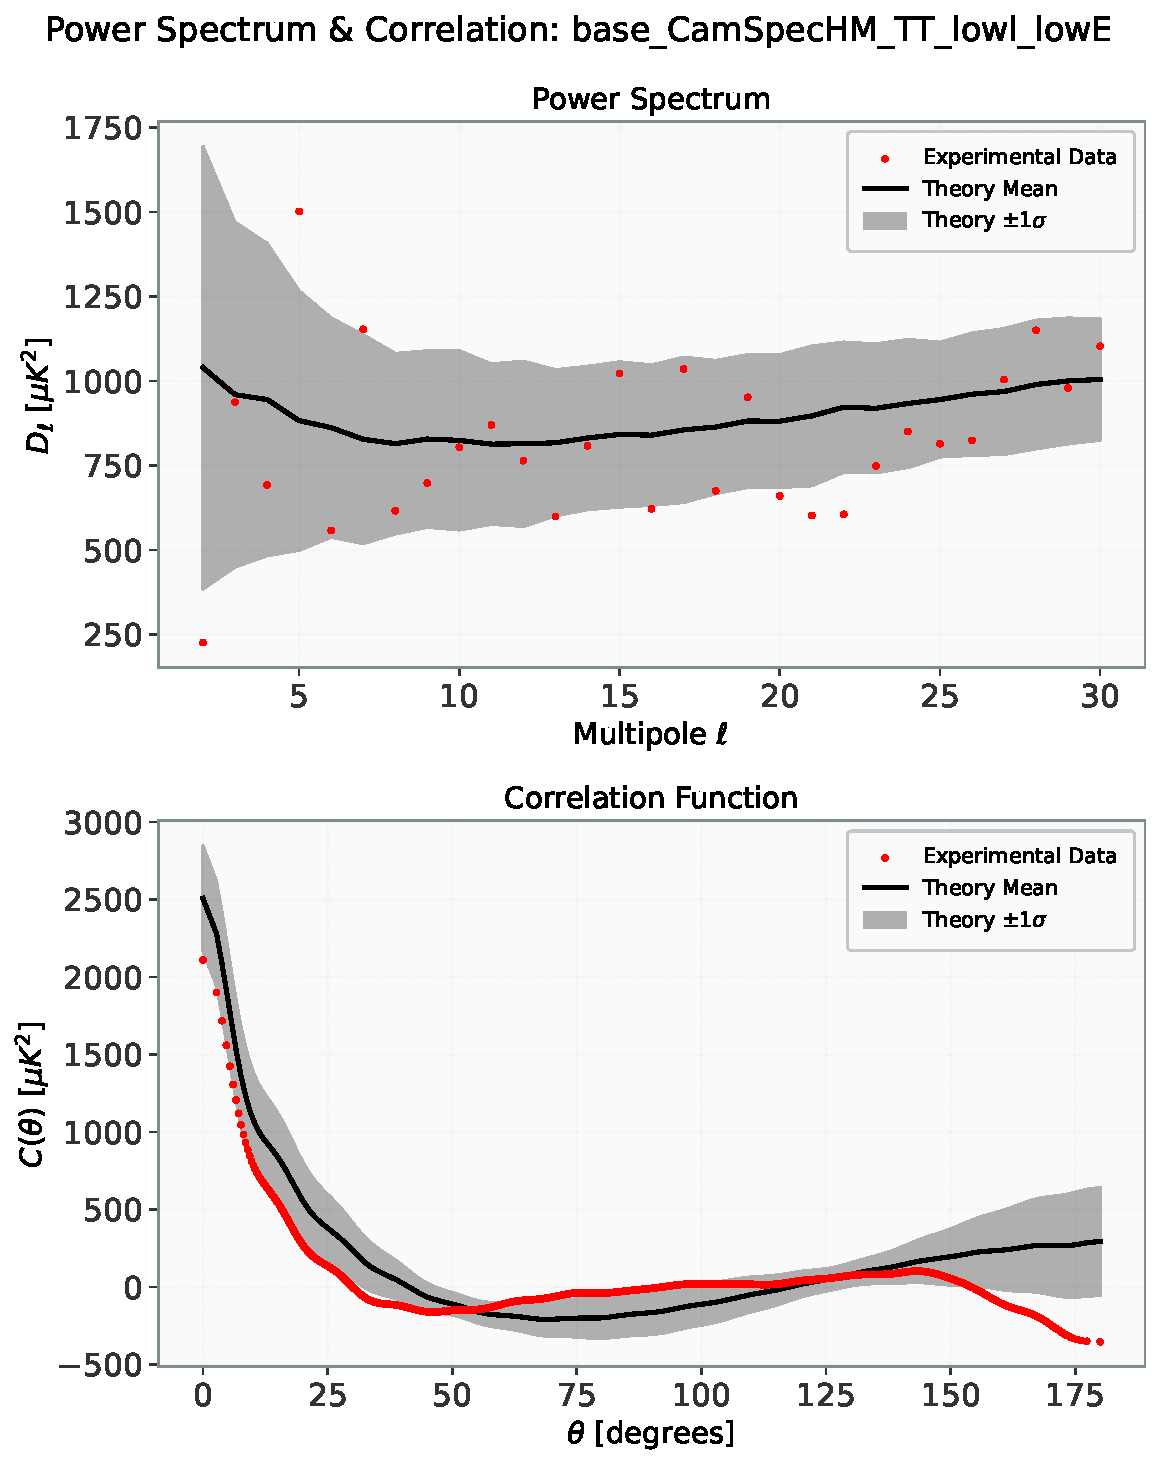
\includegraphics[width=1\linewidth,height=\textheight,keepaspectratio]{../runs/run_30_1000_all_8e4057ec/images_bestfit/powerspectrum/base_CamSpecHM_TT_lowl_lowE_power_corr.pdf}

}

\caption{Power spectrum (top) and angular correlation function (bottom)
for model \texttt{base\_CamSpecHM\_TT\_lowl\_lowE}. Experimental Planck
data (red points), theoretical mean (black line), and \(\pm 1\sigma\)
band (grey) are shown. The suppression of \(C(\theta)\) for
\(\theta \gtrsim 60°\) relative to the theoretical expectation is
visible in the lower panel.}

\end{figure}%

Both questions have rarely been addressed simultaneously in the
literature. Here we do so using Planck 2018 legacy chains: we construct
the theoretical sampling distribution by two independent methods and
combine the resulting p-values with the ACAT procedure
\citep{Liu02012020}, which accounts for the correlations among all
statistics tested and yields a single global significance.

In this work we re-examine these statistics using Planck legacy chains
and two complementary methods to construct the theoretical sampling
distribution. We focus on three statistics defined over five angular
intervals that partition the accessible range \([0°, 180°]\): the
quadratic statistic \(S_a^b\), the linear statistic
\(\langle\xi\rangle_a^b\), and the antipodal correlation \(C_{180}\).

The primary model considered throughout is the standard flat
\(\Lambda\)CDM fit to the Planck temperature power spectrum using the
CamSpec high-multipole TT likelihood combined with the low-\(\ell\)
temperature and polarization likelihoods \citep{cosmoplanck_2020}.
Results for the Plik-based likelihood and for models with free curvature
\(\Omega_k\) are reported in the appendix.

\section{Statistics}\label{sec-stats}

\FloatBarrier

The statistics studied here are designed to probe complementary aspects
of the large-angle correlation function: its integrated power, its mean
level over specific angular ranges, and its value at antipodal
separation. The choice is guided by the existing literature on
low-\(\ell\) anomalies, though as noted by \citet{Efstathiou_2010}, some
statistics , including \(S_{1/2}\) , were identified a posteriori from
the data, which inflates their apparent significance. Studying multiple
statistics simultaneously, and combining their p-values through a global
test, is therefore essential to obtain a reliable assessment of tension
with \(\Lambda\)CDM.

\subsection{Angular Power Spectrum and Correlation
Function}\label{sec-corr}

\FloatBarrier

The CMB temperature anisotropy \(\Delta T(\hat{n})/T_0\) is expanded in
spherical harmonics with coefficients \(a_{\ell m}\). For a
statistically isotropic Gaussian field the two-point statistics are
fully encoded in the angular power spectrum
\(C_\ell = \langle |a_{\ell m}|^2 \rangle\). We work with the
conventional scaled spectrum \(D_\ell = \ell(\ell+1)C_\ell/(2\pi)\),
which is approximately flat for a scale-invariant primordial spectrum.

The angular two-point correlation function is obtained by transforming
back to real space via a Legendre expansion,

\begin{equation}\phantomsection\label{eq-corr}{
C(\theta) = \sum_\ell \frac{2\ell+1}{4\pi} C_\ell P_\ell(\cos\theta)
= \sum_\ell \frac{2\ell+1}{2\ell(\ell+1)} D_\ell P_\ell(\cos\theta),
}\end{equation}

where \(P_\ell\) are Legendre polynomials. The sum runs from
\(\ell = 2\) to \(\ell_{\max} = 30\) throughout this work.

\subsection{Interval Statistics}\label{sec-statistics}

\FloatBarrier

Three statistics are evaluated on each of the angular intervals listed
in Table\textasciitilde{}\ref{tbl-intervals}, chosen to partition the
accessible range \([0°, 180°]\) into physically motivated regions while
including the classic \(S_{1/2}\) interval for comparison with the
literature.

\textbf{Antipodal correlation} \(C_{180} \equiv C(\theta = 180°)\)
measures the correlation between antipodal points on the sky. Because it
is a pointwise evaluation of \(C(\theta)\) it is relatively insensitive
to masking effects at intermediate scales, and it provides a direct test
of the near-vanishing of large-angle correlations at the largest
possible separation.

\textbf{Interval-averaged correlation} \(\langle\xi\rangle_a^b\) is the
mean of \(C(\theta)\) over the angular interval
\([\theta_a, \theta_b]\), expressed in terms of \(\mu = \cos\theta\) as

\[
\langle\xi\rangle_a^b = \frac{1}{b-a}\int_a^b C(\theta)\,d\mu
= \]
\begin{equation}\phantomsection\label{eq-xiv}{\sum_\ell \frac{D_\ell}{2\ell(\ell+1)}\,
\frac{P_{\ell+1}(b) - P_{\ell-1}(b) - P_{\ell+1}(a) + P_{\ell-1}(a)}{b-a},
}\end{equation}

where \(a = \cos\theta_b\) and \(b = \cos\theta_a\). Being linear in
\(D_\ell\), this statistic is sensitive to shifts in the mean
correlation level within an interval and changes sign when the
correlation function crosses zero, making it complementary to \(S_a^b\).

\textbf{Integrated squared correlation} \(S_a^b\) is defined as

\begin{equation}\phantomsection\label{eq-s12}{
S_a^b = \int_a^b C^2(\theta)\,\sin\theta\,d\theta
= \sum_{n,m} A_n A_m D_n D_m\, T_{nm},
}\end{equation}

where \(A_\ell = (2\ell+1)/[2\ell(\ell+1)]\) and

\[
T_{nm} =\] \[ \sum_{r=0}^{\min(m,n)}
\frac{A_r A_{m-r} A_{n-r}
\left[\Delta P_{m+n-2r+1} - \Delta P_{m+n-2r-1}\right]_a^b}
{A_{m+n-r}(2m+2n-2r+1)}
\]

are overlap integrals of Legendre polynomials over the interval
\citep{Carlitz1961}. Being quadratic in \(D_\ell\), this statistic
amplifies deviations that are coherent across multipoles and is always
non-negative, so it cannot be cancelled by sign changes of \(C(\theta)\)
within the interval. The classic \(S_{1/2}\) statistic of
\citet{Spergel_2003} corresponds to the choice
\([\theta_a, \theta_b] = [60°, 180°]\).

\begin{table}

\caption{\label{tbl-intervals}Angular intervals used for $S_a^b$ and $\langle\xi\rangle_a^b$.}

\centering{

\centering


\begin{tabular}{lll}
\toprule
Angular range & Description & $[\cos\theta_b,\;\cos\theta_a]$ \\
\midrule
$[0°,\;30°]$   & Small angles      & $[0.865,\ 1.000]$  \\
$[30°,\;92°]$  & Intermediate      & $[-0.039,\ 0.865]$ \\
$[92°,\;154°]$ & Large angles      & $[-0.901,\ -0.039]$\\
$[154°,\;180°]$& Near-antipodal    & $[-1.000,\ -0.901]$\\
$[60°,\;180°]$ & Classic $S_{1/2}$ & $[-1.000,\ 0.500]$ \\
\bottomrule
\end{tabular}

}

\end{table}%

\section{Data}\label{sec-data}

\FloatBarrier

\subsection{Planck Posterior Chains}\label{sec-planck}

\FloatBarrier

We use the publicly available Planck 2018 MCMC chains from the Planck
Legacy Archive\footnote{\url{https://pla.esac.esa.int/}}
\citep{planck_legacy_archive}. The primary dataset is the CamSpec
high-multipole TT likelihood combined with the low-\(\ell\) temperature
and polarization likelihoods (\texttt{base\_CamSpecHM\_TT\_lowl\_lowE}).
This provides posterior samples of the six standard \(\Lambda\)CDM
parameters \(\{\Omega_b h^2,\,\Omega_c h^2,\,H_0,\,\tau,\,n_s,\,A_s\}\)
along with a suite of derived quantities. The Plik-based TT likelihood
and two curvature-extended runs are considered in
Appendix\textasciitilde{}\ref{sec-appendix-tables}.

For each posterior sample the theoretical power spectrum \(D_\ell\) is
computed with CAMB \citep{CAMB_GitHub}, and the corresponding
\(C(\theta)\) and derived statistics are evaluated analytically using
equations \ref{eq-corr}--\ref{eq-s12}.

\subsection{Observed Planck Multipoles}\label{sec-obs}

\FloatBarrier

The experimental values of each statistic are computed from the Planck
2018 Commander temperature map and associated beam and pixel window
functions, using the same multipole range \(\ell \in [2, 30]\). These
observed values serve as the reference against which the theoretical
distributions are compared.

\subsection{Ensemble Construction}\label{sec-ensemble}

\FloatBarrier

Two independent strategies are used to construct the theoretical
sampling distribution.\footnote{The full analysis pipeline is publicly
  available at \url{https://github.com/PhyAMR/CMB}.}

\begin{enumerate}
\def\labelenumi{\arabic{enumi}.}
\item
  \textbf{MCMC ensemble.} For each of the 1000 samples drawn from the
  tail of the Planck posterior chain , specifically the last 1000 rows
  after GetDist's default burn-in removal , the cosmological parameters
  are passed to CAMB to compute a theoretical spectrum
  \(D_\ell^\mathrm{th}\). Each spectrum is then passed through the
  simulation pipeline described below, producing one realisation of
  cosmic variance on top of the parameter-determined
  \(D_\ell^\mathrm{th}\). The resulting ensemble therefore captures both
  parameter uncertainty and cosmic variance simultaneously, constituting
  a Bayesian predictive distribution for each statistic.
\item
  \textbf{Best-fit ensemble.} The best-fit \(D_\ell^\mathrm{bf}\) is
  read from the \texttt{.minimum.theory\_cl} file of the Planck chain,
  which contains the spectrum evaluated at the maximum-posterior
  parameter point. This single spectrum is used as input to 1000
  independent pipeline realisations, each with a different random seed.
  The spread of the resulting ensemble is driven entirely by cosmic
  variance at fixed cosmological parameters, with no contribution from
  parameter uncertainty. The width of its histograms is therefore a
  lower bound on the total variance: the additional width seen in the
  MCMC histograms is attributable purely to parameter uncertainty, and
  comparing the two ensembles provides a clean decomposition of the two
  contributions.
\end{enumerate}

In both cases, the pipeline follows the methodology of
\citet{sullivan2024methodscmbmapanalysis}. For each theoretical
\(C_\ell^\mathrm{th}\) spectrum, the beam transfer function \(b_\ell\)
and the HEALPix pixel window function \(p_\ell\) are applied, a full-sky
temperature map is synthesised at \(N_\mathrm{side} = 2048\) using
\texttt{hp.synfast}, and the pseudo-\(C_\ell\) are recovered with
\texttt{hp.anafast}. The recovered spectrum is then deconvolved by
\(b_\ell^2 p_\ell^2\) to obtain an estimate \(\hat{D}_\ell\) in the same
space as the published Planck values. When a sky mask is applied, the
recovered \(C_\ell\) are corrected by the sky fraction
\(f_\mathrm{sky}\) before deconvolution. Simulations were run both with
the Planck 2018 common mask and without any mask; results for both cases
are reported. At \(\ell_\mathrm{max} = 30\) the beam and pixel window
corrections are numerically negligible, but they are included for
consistency with the Planck data reduction.

In order to reduce the look-elsewhere effect and obtain a calibrated
global significance that accounts for the correlation structure of the
statistics without requiring an explicit model of it, we use the
Aggregated Cauchy Association Test \citep[ACAT;][]{Liu02012020}. The
eleven statistics examined , five intervals each for \(S_a^b\) and
\(\langle\xi\rangle_a^b\), plus \(C_{180}\) , are not independent: all
derive from the same realisation of \(D_\ell\), so their p-values are
correlated by construction. Treating them as independent and applying a
simple Bonferroni correction would be overly conservative, while
reporting only the most extreme individual p-value would be
anti-conservative.

For each statistic \(k \in \{1, \dots, 11\}\) the individual p-value
\(p_k\) is computed as the two-sided empirical quantile of the observed
value within the simulated ensemble: \(p_k = 2\min(F_k, 1 - F_k)\),
where \(F_k\) is the fraction of realisations with a statistic value
less than or equal to the observed one. The ACAT test statistic is then

\[
T = \sum_{k=1}^{11} w_k \tan\!\left[\left(\tfrac{1}{2} - p_k\right)\pi\right],
\]

where equal weights \(w_k = 1/11\) are used, reflecting no a priori
preference for any particular angular interval or statistic. Under the
null hypothesis, \(T\) follows a standard Cauchy distribution regardless
of the dependence structure among the \(p_k\), so the combined p-value
is obtained analytically as

\[
p_\mathrm{global} = \tfrac{1}{2} - \frac{\arctan T}{\pi}.
\]

The Cauchy combination is exact under arbitrary dependence, including
the strong correlations expected between statistics computed over
overlapping angular ranges. The global tension in units of Gaussian
standard deviations is reported as
\(n_\sigma = \Phi^{-1}(1 - p_\mathrm{global}/2)\), where \(\Phi^{-1}\)
is the probit function.

\section{Results}\label{results}

\FloatBarrier

\subsection{Best-Fit Analysis}\label{sec-bestfit}

\FloatBarrier

In the best-fit analysis the theoretical sampling distribution is
generated by Monte Carlo realizations of the CMB sky drawn from the
best-fit CamSpec \(\Lambda\)CDM spectrum. This approach isolates cosmic
variance from parameter uncertainty.

Figures \ref{fig-hist-bestfit-s12} and \ref{fig-hist-bestfit-xiv}
display the distributions of the \(S_a^b\) and \(\langle\xi\rangle_a^b\)
statistics respectively, for all five angular intervals. Each panel
shows the distribution over the 1000 Monte Carlo realizations (blue
histogram), and the observed Planck value (red vertical line).
Figure\textasciitilde{}\ref{fig-hist-bestfit-c180} shows the analogous
distribution for \(C_{180}\).

\begin{figure*}[htbp]
\centering
\begin{subfigure}[b]{0.45\textwidth}
  \includegraphics[width=\textwidth]{../runs/run_30_1000_all_8e4057ec/images_bestfit/histograms/base_CamSpecHM_TT_lowl_lowE_hist_s12-180-60.pdf}
  \caption{${S}_{60}^{180}$ (classic $S_{1/2}$)}
\end{subfigure}
\hfill
\begin{subfigure}[b]{0.45\textwidth}
  \includegraphics[width=\textwidth]{../runs/run_30_1000_all_8e4057ec/images_bestfit/histograms/base_CamSpecHM_TT_lowl_lowE_hist_s12-180-154.pdf}
  \caption{${S}_{154}^{180}$}
\end{subfigure}

\vspace{0.5em}

\begin{subfigure}[b]{0.45\textwidth}
  \includegraphics[width=\textwidth]{../runs/run_30_1000_all_8e4057ec/images_bestfit/histograms/base_CamSpecHM_TT_lowl_lowE_hist_s12-154-92.pdf}
  \caption{${S}_{92}^{154}$}
\end{subfigure}
\hfill
\begin{subfigure}[b]{0.45\textwidth}
  \includegraphics[width=\textwidth]{../runs/run_30_1000_all_8e4057ec/images_bestfit/histograms/base_CamSpecHM_TT_lowl_lowE_hist_s12-92-30.pdf}
  \caption{${S}_{30}^{92}$}
\end{subfigure}

\vspace{0.5em}

\begin{subfigure}[b]{0.45\textwidth}
  \includegraphics[width=\textwidth]{../runs/run_30_1000_all_8e4057ec/images_bestfit/histograms/base_CamSpecHM_TT_lowl_lowE_hist_s12-30-0.pdf}
  \caption{${S}_{0}^{30}$}
\end{subfigure}

\caption{Best-fit Monte Carlo distributions of the $S_a^b$ statistic for model
\texttt{base\_CamSpecHM\_TT\_lowl\_lowE} ($\ell_{\max} = 30$). Each panel shows
the normalized histogram of 1000 realizations; the red line marks the
observed Planck value. The x-axis is in logarithmic scale.}
\label{fig-hist-bestfit-s12}
\end{figure*}

As we can see, for the different intervals all values of \(S_a^b\) are
below the median of the distribution, which is not only consistent with
the lack of large-angle correlations but also suggests that tha lack is
not only present at large angles but also at intermediate and small
angles. Nvertheless, the observed values are not in the extreme tails of
the distributions, and the empirical p-values are not low enough to
claim a significant tension with \(\Lambda\)CDM.

\begin{figure*}[htbp]
\centering
\begin{subfigure}[b]{0.45\textwidth}
  \includegraphics[width=\textwidth]{../runs/run_30_1000_all_8e4057ec/images_bestfit/histograms/base_CamSpecHM_TT_lowl_lowE_hist_xiv-180-60.pdf}
  \caption{$\langle\xi\rangle_{60}^{180}$}
\end{subfigure}
\hfill
\begin{subfigure}[b]{0.45\textwidth}
  \includegraphics[width=\textwidth]{../runs/run_30_1000_all_8e4057ec/images_bestfit/histograms/base_CamSpecHM_TT_lowl_lowE_hist_xiv-180-154.pdf}
  \caption{$\langle\xi\rangle_{154}^{180}$}
\end{subfigure}

\vspace{0.5em}

\begin{subfigure}[b]{0.45\textwidth}
  \includegraphics[width=\textwidth]{../runs/run_30_1000_all_8e4057ec/images_bestfit/histograms/base_CamSpecHM_TT_lowl_lowE_hist_xiv-154-92.pdf}
  \caption{$\langle\xi\rangle_{92}^{154}$}
\end{subfigure}
\hfill
\begin{subfigure}[b]{0.45\textwidth}
  \includegraphics[width=\textwidth]{../runs/run_30_1000_all_8e4057ec/images_bestfit/histograms/base_CamSpecHM_TT_lowl_lowE_hist_xiv-92-30.pdf}
  \caption{$\langle\xi\rangle_{30}^{92}$}
\end{subfigure}

\vspace{0.5em}

\begin{subfigure}[b]{0.45\textwidth}
  \includegraphics[width=\textwidth]{../runs/run_30_1000_all_8e4057ec/images_bestfit/histograms/base_CamSpecHM_TT_lowl_lowE_hist_xiv-30-0.pdf}
  \caption{$\langle\xi\rangle_{0}^{30}$}
\end{subfigure}

\caption{Best-fit Monte Carlo distributions of the interval-averaged correlation
$\langle\xi\rangle_a^b$ for model \texttt{base\_CamSpecHM\_TT\_lowl\_lowE}.}
\label{fig-hist-bestfit-xiv}
\end{figure*}

In this set of histograms we can see that the observed values of
\(\langle\xi\rangle_a^b\) sometimes are lower and sometimes higher than
the median of the distribution, which is consistent with the fact that
\(\langle\xi\rangle_a^b\) is a linear statistic, and therefore it is
more sensitive to shifts in the mean correlation level, and the change
of sign in the correlation function in certain intervals.

\begin{figure}

\centering{

\includegraphics[width=0.7\linewidth,height=\textheight,keepaspectratio]{../runs/run_30_1000_all_8e4057ec/images_bestfit/histograms/base_CamSpecHM_TT_lowl_lowE_hist_C180.pdf}

}

\caption{\label{fig-hist-bestfit-c180}Best-fit Monte Carlo distribution
of the antipodal correlation \(C_{180}\) for model
\texttt{base\_CamSpecHM\_TT\_lowl\_lowE}.}

\end{figure}%

The statistical summary , including the median, 68\% credible interval,
observed value, and empirical p-value for each statistic , is reported
in Table\textasciitilde{}\ref{tbl-bestfit-camspec}.

\begin{table*}[h!]
\centering
\caption{Statistical summary for the best-fit analysis of model
\texttt{base\_CamSpecHM\_TT\_lowl\_lowE}. Columns give the experimental value,
best-fit median, 68\% interval, and empirical p-value.}
\label{tbl-bestfit-camspec}
\input{../runs/run_30_1000_all_8e4057ec/tables/bestfit/base_CamSpecHM_TT_lowl_lowE.tex}
\end{table*}

\subsection{MCMC Analysis}\label{sec-mcmc}

\FloatBarrier

In the MCMC analysis the theoretical sampling distribution is
constructed directly from the Planck posterior, propagating full
parameter uncertainty through to the derived statistics. The 1000
posterior samples drawn from the CamSpec \(\Lambda\)CDM chain each yield
a distinct \(D_\ell\) spectrum, whose distribution reflects both cosmic
variance and parameter degeneracies.

Figures \ref{fig-hist-mcmc-s12}, \ref{fig-hist-mcmc-xiv}, and
\ref{fig-hist-mcmc-c180} show the resulting distributions of \(S_a^b\),
\(\langle\xi\rangle_a^b\), and \(C_{180}\) respectively. The broader
width of the MCMC-derived histograms compared to the best-fit case
reflects the additional spread due to cosmological parameter
uncertainty.

\begin{figure*}[htbp]
\centering
\begin{subfigure}[b]{0.45\textwidth}
  \includegraphics[width=\textwidth]{../runs/run_30_1000_all_8e4057ec/images_mcmc/histograms/base_CamSpecHM_TT_lowl_lowE_hist_s12-180-60.pdf}
  \caption{${S}_{60}^{180}$ (classic $S_{1/2}$)}
\end{subfigure}
\hfill
\begin{subfigure}[b]{0.45\textwidth}
  \includegraphics[width=\textwidth]{../runs/run_30_1000_all_8e4057ec/images_mcmc/histograms/base_CamSpecHM_TT_lowl_lowE_hist_s12-180-154.pdf}
  \caption{${S}_{154}^{180}$}
\end{subfigure}

\vspace{0.5em}

\begin{subfigure}[b]{0.45\textwidth}
  \includegraphics[width=\textwidth]{../runs/run_30_1000_all_8e4057ec/images_mcmc/histograms/base_CamSpecHM_TT_lowl_lowE_hist_s12-154-92.pdf}
  \caption{${S}_{92}^{154}$}
\end{subfigure}
\hfill
\begin{subfigure}[b]{0.45\textwidth}
  \includegraphics[width=\textwidth]{../runs/run_30_1000_all_8e4057ec/images_mcmc/histograms/base_CamSpecHM_TT_lowl_lowE_hist_s12-92-30.pdf}
  \caption{${S}_{30}^{92}$}
\end{subfigure}

\vspace{0.5em}

\begin{subfigure}[b]{0.45\textwidth}
  \includegraphics[width=\textwidth]{../runs/run_30_1000_all_8e4057ec/images_mcmc/histograms/base_CamSpecHM_TT_lowl_lowE_hist_s12-30-0.pdf}
  \caption{${S}_{0}^{30}$}
\end{subfigure}

\caption{MCMC posterior distributions of the $S_a^b$ statistic for model
\texttt{base\_CamSpecHM\_TT\_lowl\_lowE}. Each panel shows the distribution
over 1000 posterior samples from the Planck CamSpec chain.}
\label{fig-hist-mcmc-s12}
\end{figure*}

\begin{figure*}[htbp]
\centering
\begin{subfigure}[b]{0.45\textwidth}
  \includegraphics[width=\textwidth]{../runs/run_30_1000_all_8e4057ec/images_mcmc/histograms/base_CamSpecHM_TT_lowl_lowE_hist_xiv-180-60.pdf}
  \caption{$\langle\xi\rangle_{60}^{180}$}
\end{subfigure}
\hfill
\begin{subfigure}[b]{0.45\textwidth}
  \includegraphics[width=\textwidth]{../runs/run_30_1000_all_8e4057ec/images_mcmc/histograms/base_CamSpecHM_TT_lowl_lowE_hist_xiv-180-154.pdf}
  \caption{$\langle\xi\rangle_{154}^{180}$}
\end{subfigure}

\vspace{0.5em}

\begin{subfigure}[b]{0.45\textwidth}
  \includegraphics[width=\textwidth]{../runs/run_30_1000_all_8e4057ec/images_mcmc/histograms/base_CamSpecHM_TT_lowl_lowE_hist_xiv-154-92.pdf}
  \caption{$\langle\xi\rangle_{92}^{154}$}
\end{subfigure}
\hfill
\begin{subfigure}[b]{0.45\textwidth}
  \includegraphics[width=\textwidth]{../runs/run_30_1000_all_8e4057ec/images_mcmc/histograms/base_CamSpecHM_TT_lowl_lowE_hist_xiv-92-30.pdf}
  \caption{$\langle\xi\rangle_{30}^{92}$}
\end{subfigure}

\vspace{0.5em}

\begin{subfigure}[b]{0.45\textwidth}
  \includegraphics[width=\textwidth]{../runs/run_30_1000_all_8e4057ec/images_mcmc/histograms/base_CamSpecHM_TT_lowl_lowE_hist_xiv-30-0.pdf}
  \caption{$\langle\xi\rangle_{0}^{30}$}
\end{subfigure}

\caption{MCMC posterior distributions of $\langle\xi\rangle_a^b$ for model
\texttt{base\_CamSpecHM\_TT\_lowl\_lowE}.}
\label{fig-hist-mcmc-xiv}
\end{figure*}

\begin{figure}

\centering{

\includegraphics[width=0.7\linewidth,height=\textheight,keepaspectratio]{../runs/run_30_1000_all_8e4057ec/images_mcmc/histograms/base_CamSpecHM_TT_lowl_lowE_hist_C180.pdf}

}

\caption{\label{fig-hist-mcmc-c180}MCMC posterior distribution of
\(C_{180}\) for model \texttt{base\_CamSpecHM\_TT\_lowl\_lowE}.}

\end{figure}%

The quantitative results for the MCMC ensemble are collected in
Table\textasciitilde{}\ref{tbl-mcmc-camspec}.

\begin{table*}[h!]
\centering
\caption{Statistical summary for the MCMC analysis of model
\texttt{base\_CamSpecHM\_TT\_lowl\_lowE}. Columns give the experimental value,
MCMC median, 68\% credible interval, and empirical p-value.}
\label{tbl-mcmc-camspec}
\input{../runs/run_30_1000_all_8e4057ec/tables/mcmc/base_CamSpecHM_TT_lowl_lowE.tex}
\end{table*}

\section{Discussion}\label{sec-discussion}

\FloatBarrier

The results for alternative likelihoods and models with free curvature
\(\Omega_k\) are reported in
Appendix\textasciitilde{}\ref{sec-appendix-tables}. The dependence of
the results on the likelihood choice (CamSpec vs.~Plik) provides a
useful cross-check, while the curvature-extended models test whether a
departure from flatness could alleviate the observed tensions.

As noted in \citep{Efstathiou_2010}, in the low-\(\ell\) regime, the
theoretical distribution of the statistics is mostly independent of the
mask used, and the effects of the mask are negligible.

\section{Conclusions}\label{sec-conclusions}

\FloatBarrier

We have studied the large-angle CMB angular correlation function and its
derived statistics using Planck 2018 data and two complementary
ensembles for the theoretical sampling distributions. The statistics
examined , the quadratic \(S_a^b\), the linear
\(\langle\xi\rangle_a^b\), and the antipodal \(C_{180}\) --- probe
distinct aspects of the large-angle temperature field.

Both ensembles provide complementary perspectives on the significance of
the large-angle anomalies. The best-fit ensemble isolates the
contribution of cosmic variance, while the MCMC ensemble captures the
full parameter uncertainty and the cosmic variance.

A complete summary of all p-values and multivariate tension estimates
for the primary \texttt{base\_CamSpecHM\_TT\_lowl\_lowE} model is
provided in Tables\textasciitilde{}\ref{tbl-bestfit-camspec} and
\ref{tbl-mcmc-camspec}; results for additional models appear in
Appendix\textasciitilde{}\ref{sec-appendix-tables}.

While the lack of large-angle correlations is a persistent feature of
the observed CMB sky, specially the \(C_{180}\) statistic, the
\(\Lambda\)CDM model is not in significant tension with the data when
the full distribution of statistics is taken into account. The observed
values are generally below the median of the theoretical distributions,
consistent with the lack of large-angle correlations.

Another raised question from previous analyses is whether the lack of
large-angle correlations is a statistical fluke or a hint of new
physics. The observed p-values for the \(C_{180}\) statistic are low
accross multiple simulations and models, and while they are in the order
of 2-2.5\(\sigma\) the fact that it is persistent accross all our
simulations makes it more clear that the lack of large-angle
correlations is a real feature of the data, and not a statistical fluke.

\section*{References}\label{references}
\addcontentsline{toc}{section}{References}

\renewcommand{\bibsection}{}
\bibliography{main.bib}

\appendix

\FloatBarrier

\section{Additional Models: Statistical
Tables}\label{sec-appendix-tables}

The tables in this appendix report the full statistical summary for
three additional Planck models. All quantities are defined as in the
main text. Model names follow the Planck convention: \texttt{omegak}
denotes a run with free spatial curvature; \texttt{plikHM} denotes the
Plik high-multipole likelihood; \texttt{TTTEEE} denotes a joint
temperature and polarization fit.

\FloatBarrier

\subsection{No masked sky}\label{sec-appendix-nomask}

In this section the theoretical sampling distributions are constructed
without applying any sky mask, so the recovered \(C_\ell\) are not
corrected by \(f_\mathrm{sky}\) before deconvolution. The observed
values are computed from the full-sky Commander map, so they are
directly comparable to the theoretical distributions without any
correction for masking effects.

\FloatBarrier

\subsubsection{MCMC Results}\label{sec-app-mcmc}

\begin{table*}[h!]
\centering
\caption{MCMC results for \texttt{base\_plikHM\_TT\_lowl\_lowE}.}
\input{../runs/run_30_1000_all_8e4057ec/tables/mcmc/base_plikHM_TT_lowl_lowE.tex}
\end{table*}

\begin{table*}[h!]
\centering
\caption{MCMC results for \texttt{base\_omegak\_CamSpecHM\_TT\_lowl\_lowE}.}
\input{../runs/run_30_1000_all_8e4057ec/tables/mcmc/base_omegak_CamSpecHM_TT_lowl_lowE.tex}
\end{table*}

\begin{table*}[h!]
\centering
\caption{MCMC results for \texttt{base\_omegak\_plikHM\_TTTEEE\_lowl\_lowE}.}
\input{../runs/run_30_1000_all_8e4057ec/tables/mcmc/base_omegak_plikHM_TTTEEE_lowl_lowE.tex}
\end{table*}

\FloatBarrier

\subsubsection{Best-Fit Results}\label{sec-app-bestfit}

\begin{table*}[h!]
\centering
\caption{Best-fit results for \texttt{base\_plikHM\_TT\_lowl\_lowE}.}
\input{../runs/run_30_1000_all_8e4057ec/tables/bestfit/base_plikHM_TT_lowl_lowE.tex}
\end{table*}

\begin{table*}[h!]
\centering
\caption{Best-fit results for \texttt{base\_omegak\_CamSpecHM\_TT\_lowl\_lowE}.}
\input{../runs/run_30_1000_all_8e4057ec/tables/bestfit/base_omegak_CamSpecHM_TT_lowl_lowE.tex}
\end{table*}

\begin{table*}[h!]
\centering
\caption{Best-fit results for \texttt{base\_omegak\_plikHM\_TTTEEE\_lowl\_lowE}.}
\input{../runs/run_30_1000_all_8e4057ec/tables/bestfit/base_omegak_plikHM_TTTEEE_lowl_lowE.tex}
\end{table*}

\FloatBarrier

\subsection{Masked sky}\label{sec-appendix-masked}

In this section the theoretical sampling distributions are constructed
with the Planck common mask applied, so the recovered \(C_\ell\) are
corrected by \(f_\mathrm{sky}\) before deconvolution.

\FloatBarrier

\subsubsection{MCMC Results}\label{sec-app-mcmc-masked}

\begin{table*}[h!]
\centering
\caption{MCMC results for
\texttt{base\_CamSpecHM\_TT\_lowl\_lowE} with masked sky. }
\label{tbl-mcmc-camspec-masked}
\input{../runs/run_30_1000_all_8e4057ec/tables/mcmc/base_CamSpecHM_TT_lowl_lowE.tex}
\end{table*}

\begin{table*}[h!]
\centering
\caption{MCMC results for \texttt{base\_plikHM\_TT\_lowl\_lowE} with masked sky. }
\label{tbl-mcmc-plikHM-masked}
\input{../runs/run_30_1000_all_8f075564/tables/mcmc/base_plikHM_TT_lowl_lowE.tex}
\end{table*}

\begin{table*}[h!]
\centering
\caption{MCMC results for \texttt{base\_omegak\_CamSpecHM\_TT\_lowl\_lowE} with masked sky.}
\label{tbl-mcmc-omegak-camspec}
\input{../runs/run_30_1000_all_8f075564/tables/mcmc/base_omegak_CamSpecHM_TT_lowl_lowE.tex}
\end{table*}

\begin{table*}[h!]
\centering
\caption{MCMC results for \texttt{base\_omegak\_plikHM\_TTTEEE\_lowl\_lowE} with masked sky.}
\label{tbl-mcmc-omegak-plikHM}
\input{../runs/run_30_1000_all_8f075564/tables/mcmc/base_omegak_plikHM_TTTEEE_lowl_lowE.tex}
\end{table*}

\FloatBarrier

\subsubsection{Best-Fit Results}\label{sec-app-bestfit-masked}

The mask effect for models with free curvature (\(\Omega_k\)) is not
properly captured since the mask was not designed for those models,
while in the MCMC case that effect has been mitigated by the fact that
the MCMC ensemble includes a range of cosmological parameters, so the
mask effect is averaged over the posterior distribution. In the best-fit
case, however, the cosmological parameters are fixed at the best-fit
point, so the mask effect is not averaged over the posterior
distribution, and therefore it is not properly captured. For that reason
the significance of those models with \(T\ll0\) can not be interpreted
correctly.

\begin{table*}[h!]
\centering
\caption{Best-fit results for
\texttt{base\_CamSpecHM\_TT\_lowl\_lowE} with masked sky. }
\label{tbl-bestfit-camspec-masked}
\input{../runs/run_30_1000_all_8e4057ec/tables/bestfit/base_CamSpecHM_TT_lowl_lowE.tex}
\end{table*}

\begin{table*}[h!]
\centering
\caption{Best-fit results for \texttt{base\_plikHM\_TT\_lowl\_lowE} with masked sky.}
\label{tbl-bestfit-plikHM-masked}
\input{../runs/run_30_1000_all_8f075564/tables/bestfit/base_plikHM_TT_lowl_lowE.tex}
\end{table*}

\begin{table*}[h!]
\centering
\caption{Best-fit results for \texttt{base\_omegak\_CamSpecHM\_TT\_lowl\_lowE} with masked sky.}
\label{tbl-bestfit-omegak-camspec}
\input{../runs/run_30_1000_all_8f075564/tables/bestfit/base_omegak_CamSpecHM_TT_lowl_lowE.tex}
\end{table*}

\begin{table*}[h!]
\centering
\caption{Best-fit results for \texttt{base\_omegak\_plikHM\_TTTEEE\_lowl\_lowE} with masked sky.}
\label{tbl-bestfit-omegak-plikHM}
\input{../runs/run_30_1000_all_8f075564/tables/bestfit/base_omegak_plikHM_TTTEEE_lowl_lowE.tex}
\end{table*}

\FloatBarrier





\end{document}
